%___________________________ Q 4.3 ______________________________
\subsection{Comment on the choice of the weights on the quadratic cost when using the LQG design approach. Include the root-square locus. (3 pts)}
\vspace{10pt}

%%Write your answer here

The cost function being minimized in our system is defined as shown in equation \ref{eq:cost_function}, where $Q$ and $R$ represent the weights of the quadratic cost. By adjusting these values, we effectively control the relative importance of the system's state versus the control signal. This allows us to prioritize either minimizing the state error, irrespective of the energy consumed (control signal), or reducing energy usage while accepting a larger error.

Given the state space formulation and the specific characteristics of our system—namely, that the control signal does not have an immediate effect on the output (i.e., $\text{D} = 0$)—we must set $Q = C^{T}C$. This reduces the problem to finding the optimal value for $R$ that yields the best performance.

To determine the appropriate value of $R$, we begin by examining the square root locus, as shown in figure \ref{fig:Square Root locus of the system}. At first glance, the presence of poles outside the unit circle suggests an unstable discrete-time system. However, these poles actually belong to the closed-loop system, i.e., they are the poles of $1 + G(z)G(z^{-1})$. Therefore, we are only concerned with the poles inside the unit circle, as the poles outside it are due to $G(z^{-1})$ and do not have any physical significance. Inside the unit circle, we observe a set of poles (marked in red) corresponding to the estimator. Since the controller cannot be faster than the estimator, this provides an upper bound for $R$, which, in this case, is determined by the inverse of the estimator gain—set to 1.

From this analysis, we applied a trial-and-error approach, testing multiple values of $R$. The system's response to these variations is shown in figure \ref{fig: system response variation with changes in R}. The optimal result was achieved with $R = 50$, as it minimized the delay seen with smaller values of $R$, while still reducing the system's energy consumption. It may be important for the reader to note that the system response in figure  \ref{fig: system response variation with changes in R} uses the controller present in figure \ref{fig:controler_with_integrator}, which incorporates integral action with saturation limits, the reason for this will be explained in a later question.

\begin{minipage}{0.3\textwidth}
    \fontsmall
    \begin{equation}
        J = \sum_{k=0}^{\infty} \left[ (x^{T}(k)Qx(k) + u^{T}(k)Ru(k)\right]
        \label{eq:cost_function}
    \end{equation}
\end{minipage}
\hfill
\begin{minipage}{0.75\textwidth}    
    \begin{figure}[H]
        \centering
        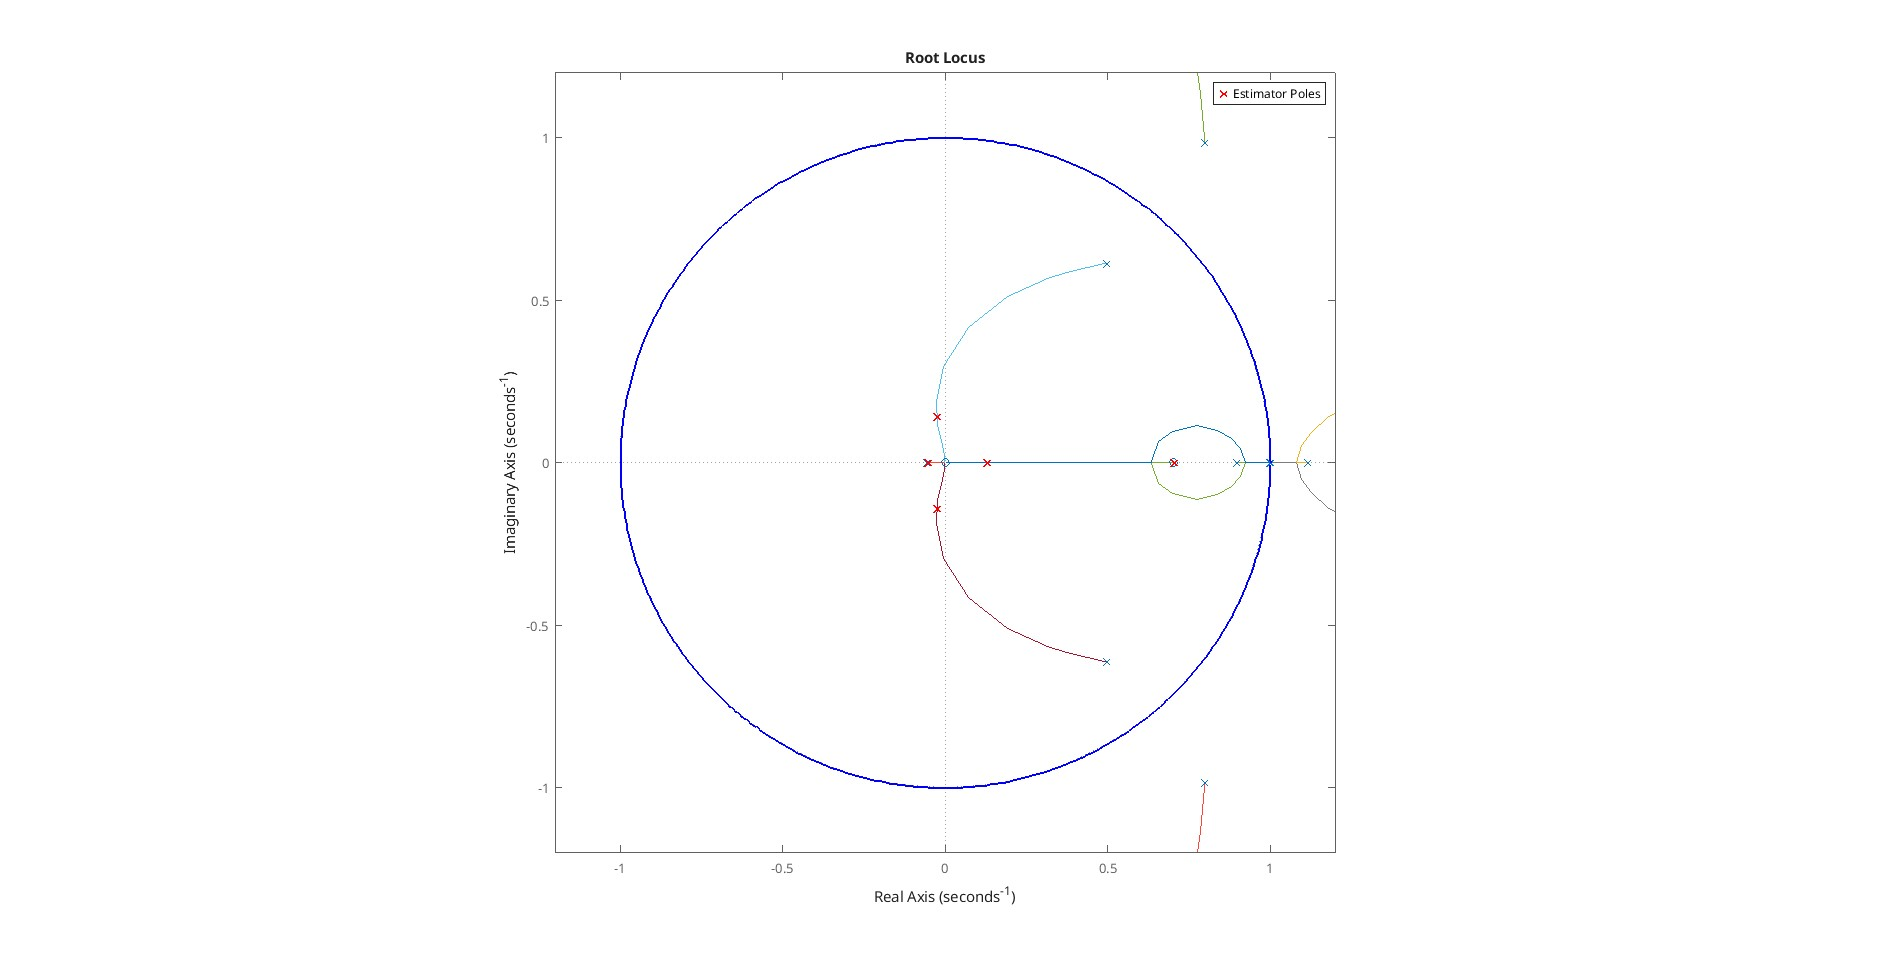
\includegraphics[width=0.94\textwidth]{Figs/root_locus.jpg}
        \caption{Root Locus}
        \label{fig:Square Root locus of the system}
    \end{figure}
\end{minipage}


\begin{figure}
    \centering
    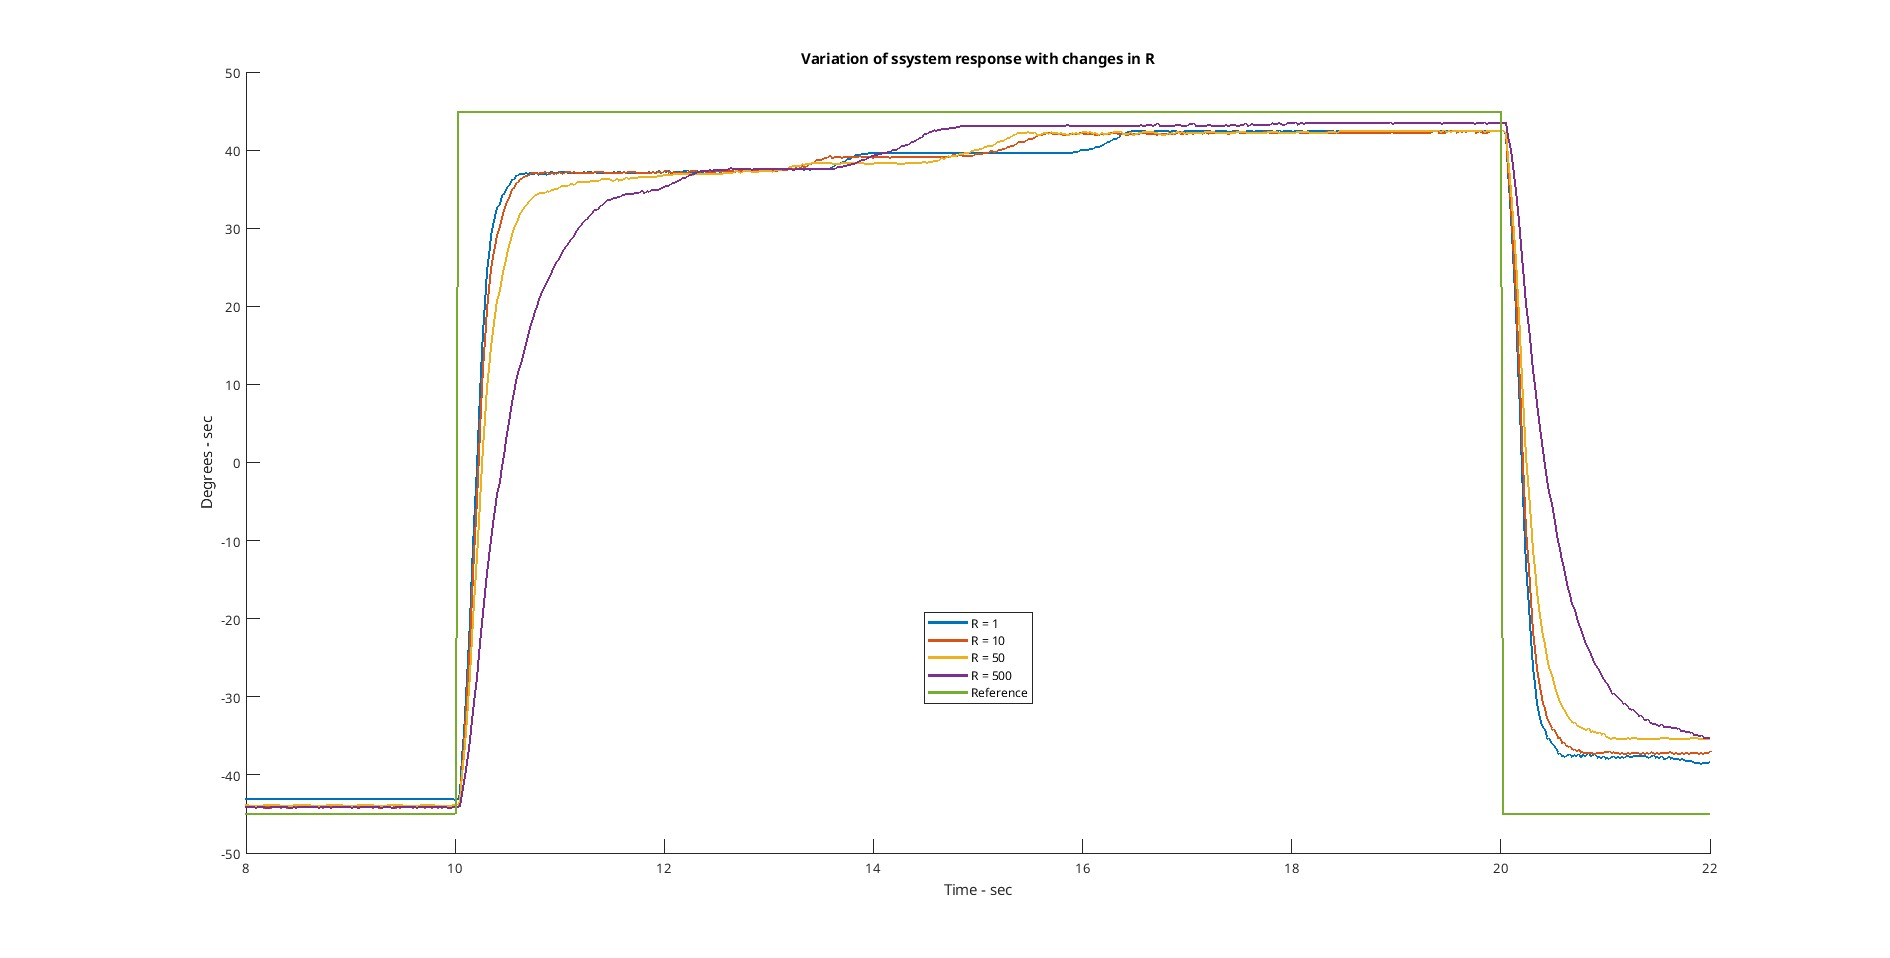
\includegraphics[width=0.6\textwidth]{Figs/system_response_variation_with_R.jpg}
    \caption{System Response variation with R}
    \label{fig: system response variation with changes in R} 
\end{figure}